\documentclass[a4paper,10pt]{beamer}
\usepackage[utf8x]{inputenc}
\usepackage[T1]{fontenc}
\usepackage[french]{babel}
\usepackage{hyperref,graphicx,multicol,eurosym,tabularx,color}
\usetheme{Berkeley}
\setbeamercolor{structure}{fg=cyan!60!black}
\setbeamercolor{navigation symbols}{fg=black}
\setbeamertemplate{navigation symbols}{\large \insertframenumber /\inserttotalframenumber}
\newcolumntype{M}[1]{>{\centering\arraybackslash}m{#1}}

\title{Création d'objets 3D à partir de dessins 2D}
\author[Groupe 3INFO]{Aurélien Fontaine, Manutea Huang,
\\ Etienne Geantet, Arnaud Martin}
\institute[INSA de Rennes]{Institut National des Sciences Appliquées de Rennes}
\date{\today}

\begin{document}
	
	\begin{frame}
		\begin{titlepage}
			\centerline{
\includegraphics[scale=0.1]{images/logos/logoINSA.jpg}}
			\centerline{Encadrants : François Lehericey et Bertrand Coüasnon}	
		\end{titlepage}
	\end{frame}
	
	\section{Introduction}
	
	\begin{frame}{Introduction}
		\begin{itemize}
		\item Un projet proposé par les chercheurs de l'Irisa.
		\end{itemize}
		\centerline{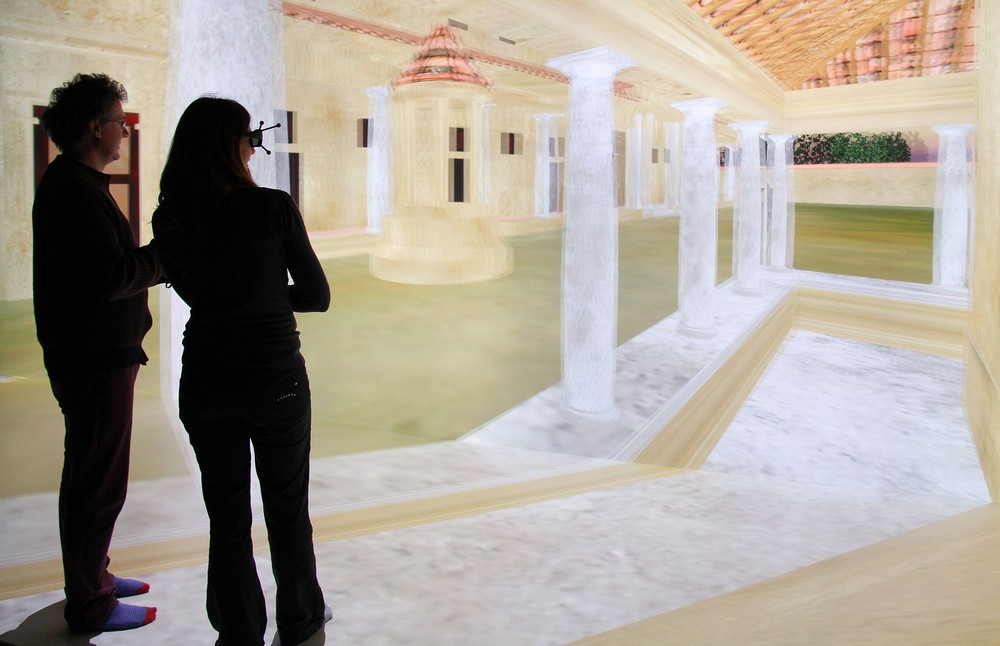
\includegraphics[scale=0.25]{images/intro/Immersia.jpg}}
		\centerline{Comment meubler rapidement une scène de réalité}
		\centerline{virtuelle avec divers objets 3D ?}
	\end{frame}
	
	\begin{frame}{Objectifs du projet}
		Contexte :
		\begin{itemize}
			\item Recherches sur la physique des objets 3D en réalité virtuelle.
			\item Besoin: Créer rapidement des modèles 3D pour les tests.\pause
		\end{itemize}
		Problème :
			\begin{itemize}
				\item Créer un objet 3D prend beaucoup de temps (au moins 1h pour un artiste).
				\item Or dans ce cas, pas besoin d'objets complexes et esthétiques !\pause
			\end{itemize}
		Notre projet :
		\begin{itemize}
		\item Permettre la \textbf{création rapide} d'objets simples à partir de dessins 2D.
		\item L'application met l'accent sur la \textbf{simplicité} d'utilisation et \textbf{l'ergonomie} plutôt que sur la qualité graphique des modèles.
		\end{itemize}
			\centerline{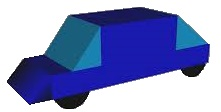
\includegraphics[scale=0.3]{images/intro/car.jpg}}
	\end{frame}
	
	\begin{frame}{Sommaire}
		\tableofcontents
	\end{frame}
	
	\section{Cahier des charges}
	
	\begin{frame}{Cahier des charges}
		Notre projet doit respecter les contraintes suivantes:
		\begin{itemize}
			\item Fonctionner sur tablette
			\item Dessiner à main levée
			\item Plusieurs outils de dessin
			\item Transformer ces dessins en objets 3D (Extrusion)
			\item Pouvoir assembler les objets 3D
			\item Application ergonomique et intuitive
			\item Exportation vers un serveur Unity
		\end{itemize}
	\end{frame}
	
	\section{Etat de l'art}
	
		\begin{frame}{Quelles technologie utiliser ?}
			\begin{tabular}{|M{45pt}|M{50pt}|M{38pt}|M{60pt}|M{30pt}|}
				\hline
				\textbf{Software} & \textbf{Facile à apprendre} & \textbf{Manipule bcp d'objets} & \textbf{Prix} & \textbf{Aide pour tablettes}\\
				\hline
			\end{tabular}
			\smallbreak
			API :
			\begin{tabular}{|M{45pt}|M{50pt}|M{38pt}|M{60pt}|M{30pt}|}
				\hline
				\textit{OpenGl} & \color{red}{$\times$} & \color{orange}{$\sim$} & \color{green}{0\euro} & \color{red}{$\times$}\\
				\hline
			\end{tabular}
			\smallbreak
			Logiciel de modélisation :
			\begin{tabular}{|M{45pt}|M{50pt}|M{38pt}|M{60pt}|M{30pt}|}
				\hline
				\textit{Autodesk Maya} & \color{red}{$\times$} & \color{green}{\checkmark} & \color{red}{\$185.00/mois} & \color{orange}{$\sim$}\\
				\hline
			\end{tabular}
			\smallbreak
			Moteurs de jeu :
			\begin{tabular}{|M{45pt}|M{50pt}|M{38pt}|M{60pt}|M{30pt}|}
				\hline
				\textit{Unreal Engine} & \color{green}{\checkmark} & \color{green}{\checkmark} & \color{orange}5 \% & \color{red}{$\times$}\\
				\hline
				\textit{CryEngine} & \color{green}{\checkmark} & \color{green}{\checkmark} & \color{orange}{9.99\euro/mois} & \color{orange}{$\sim$}\\
				\hline
				\textit{Unity} & \color{green}{\checkmark} & \color{green}{\checkmark} & \color{green}{0\euro : licence gratuite} & \color{green}{\checkmark} \\
				\hline
			\end{tabular}
		\end{frame}
		
		\begin{frame}{Le petit plus pour Unity}
			\centerline{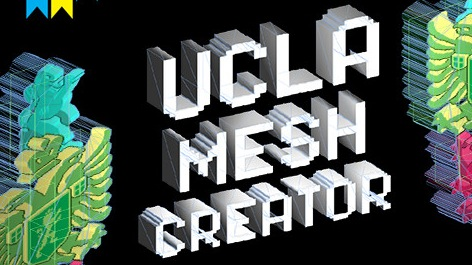
\includegraphics[height=80pt]{images/techno/ucla.jpg}}
			
			\begin{itemize}
				\item UCLA Mesh Creator : Extrusion d'un dessin 2D
					\begin{itemize}
						\item Création uniquement en mode "Edition" de Unity
						\item Ne gère pas les trous
					\end{itemize}
				\item Gros avantage : Réutilisable facilement et sans contrainte
				\item Licence très permissive
			\end{itemize}
			
		\end{frame}
		

	
	\section{Conception}	
		\begin{frame}{Conception}
		
		Deux points de réflexion:
			\begin{itemize}
				  \item Définir comment être ergonomique
				  	
				  	\begin{itemize}
				  		\item Comment organiser l'IHM?
				  		\item Comment dessiner?
				  		\item Comment extruder et placer la figure créée dans l'environnement 3D?
				  	\end{itemize}
				  \item Diviser le logiciel en éléments simples
			
			\end{itemize}
		\end{frame}
		

		
			
			\begin{frame}{Comment être ergonomique?}
				Comment organiser l'IHM?
				
				\begin{itemize}
					\item Accueillir les futurs éléments
					\item Simplicité: peu d'options, sobre
				\end{itemize}

				\centerline{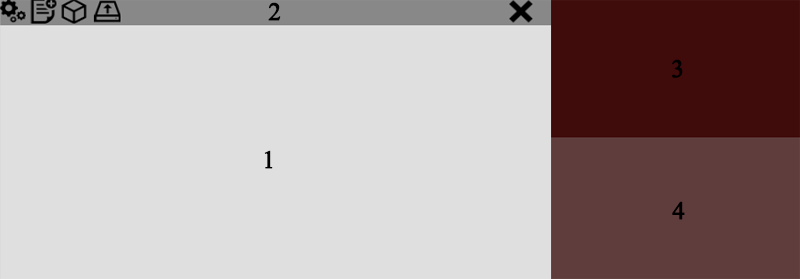
\includegraphics[scale=0.3]{images/Nono/img6.png}}
			Blender:
				\centerline{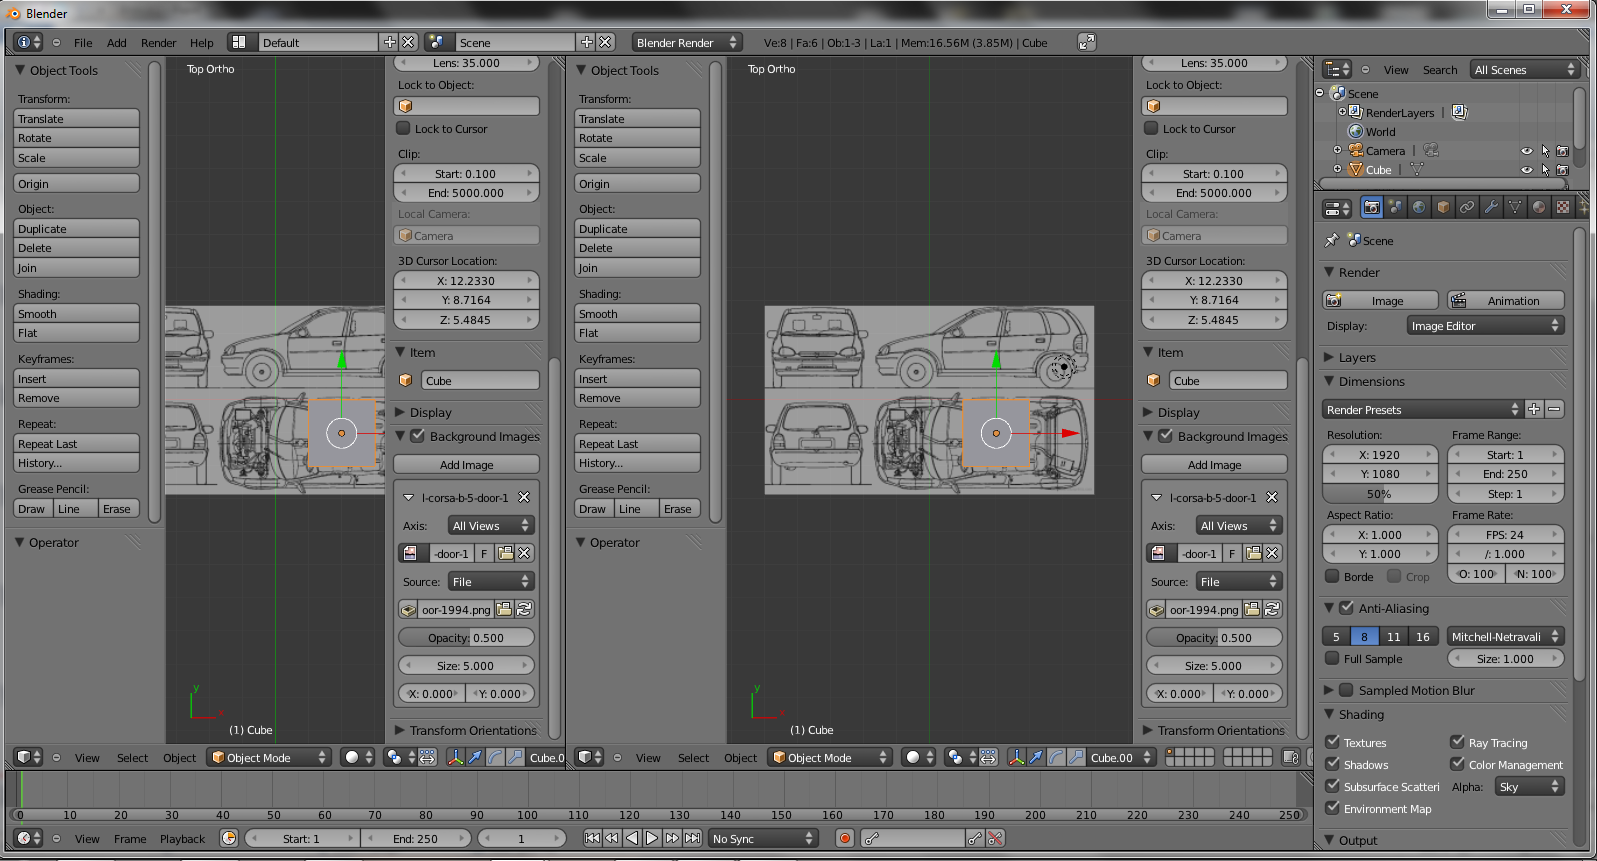
\includegraphics[scale=0.15]{images/Nono/img5.png}} 
			\end{frame}
		
		\begin{frame}{Comment être ergonomique?}

				Comment dessiner?
					\begin{itemize}
						\item Interface sobre
						\item Menu d'outils simple
					\end{itemize}
				
				\centerline{
\includegraphics[scale=0.3]{images/Nono/img1.png}} \centerline{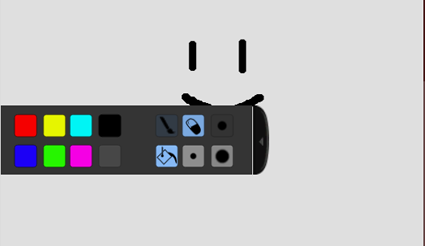
\includegraphics[scale=0.3]{images/Nono/img2.png}}
			


		\end{frame}	
		
		\begin{frame}{Comment être ergonomique?}
			
			Comment extruder et placer la figure créée dans l'environnement 3D?
			\begin{itemize}
				\item Limiter les options
				\item Découper en plusieurs étapes
				\item Transparences des autres objets
				\item Caméra globale amovible
			\end{itemize}
			
				\centerline{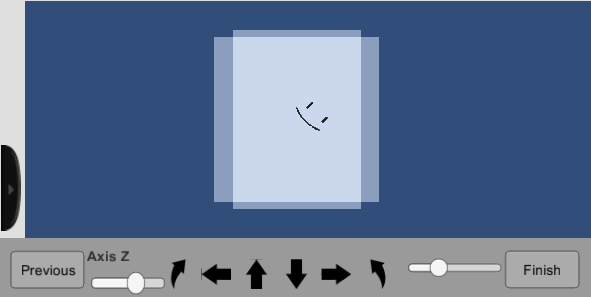
\includegraphics[scale=0.4]{images/Nono/img4.png}} 
			
			
		\end{frame}	
			
	
	\begin{frame}{Architecture logicielle} %Découpage de l'application}
		\centerline{\huge Conception modulaire de l'application}
	\end{frame}
	
	\begin{frame}{Architecture logicielle} %Découpage de l'application}
		%Archi logi Manutea
		\centerline{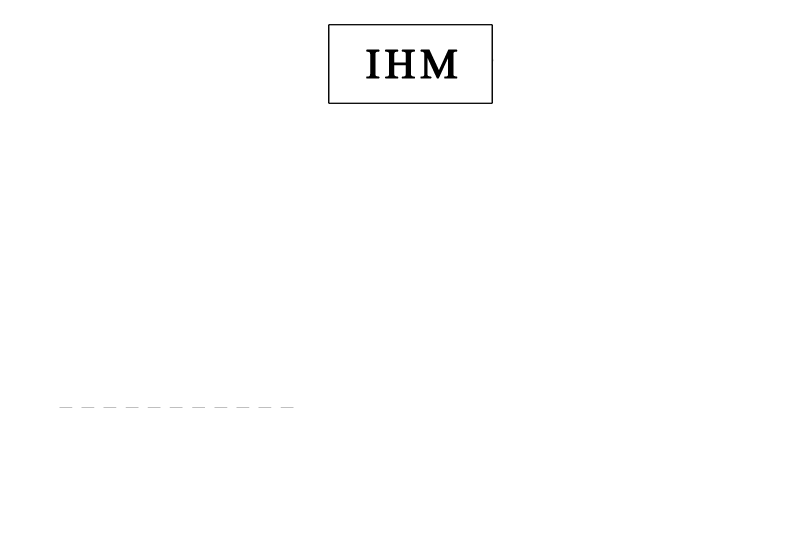
\includegraphics[scale=0.3]{images/archilogi/archi1.png}}
	\end{frame}
	\begin{frame}{Architecture logicielle} %Découpage de l'application}
		%Archi logi Manutea
		\centerline{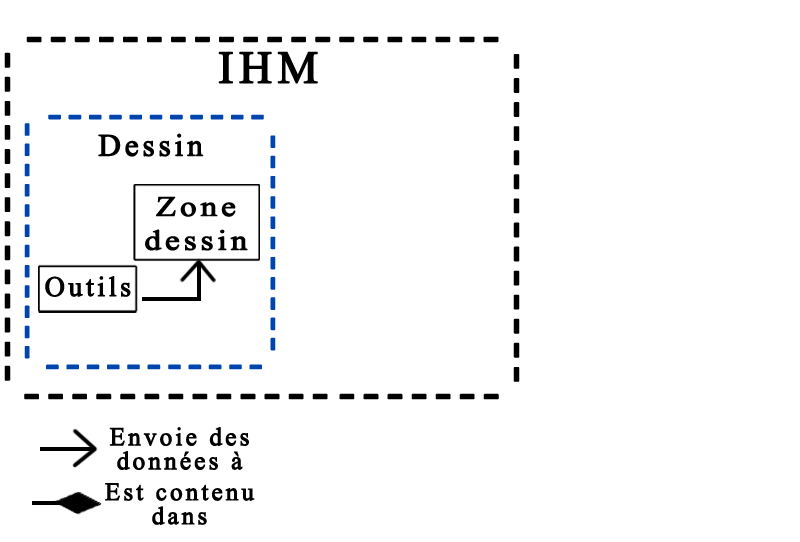
\includegraphics[scale=0.3]{images/archilogi/archi2.png}}
	\end{frame}
	\begin{frame}{Architecture logicielle} %Découpage de l'application}
		%Archi logi Manutea
		\centerline{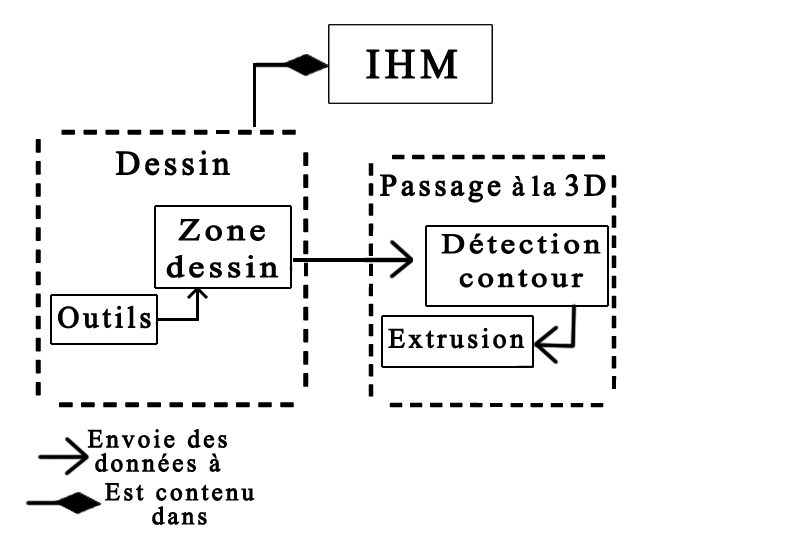
\includegraphics[scale=0.3]{images/archilogi/archi3.png}}
	\end{frame}
	\begin{frame}{Architecture logicielle} %Découpage de l'application}
		%Archi logi Manutea
		\centerline{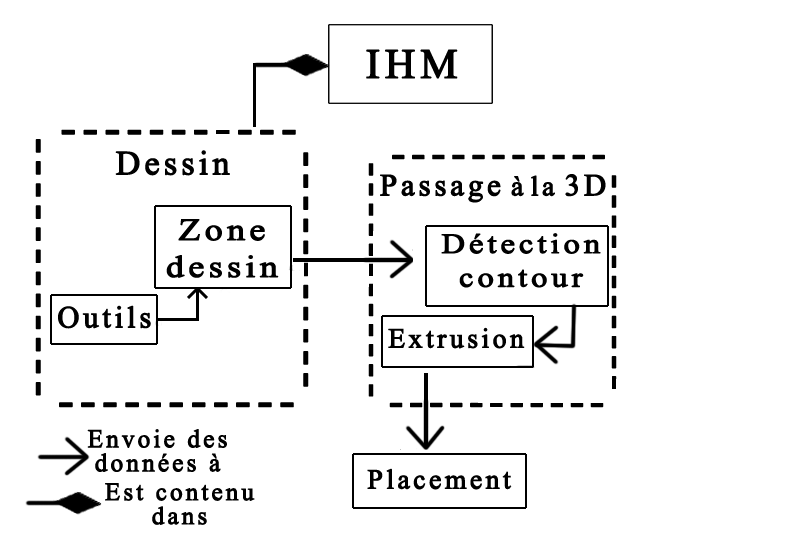
\includegraphics[scale=0.3]{images/archilogi/archi4.png}}
	\end{frame}
	\begin{frame}{Architecture logicielle} %Découpage de l'application}
		%Archi logi Manutea
		\centerline{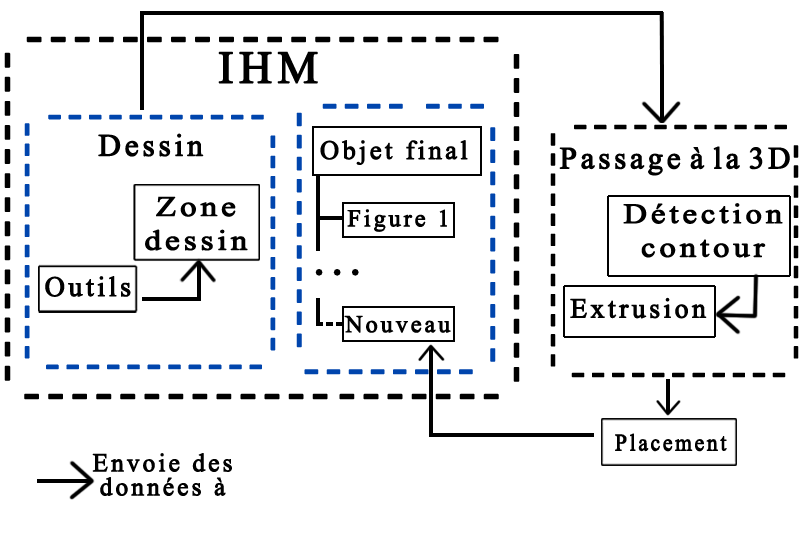
\includegraphics[scale=0.3]{images/archilogi/archi5.png}}
	\end{frame}	
	\begin{frame}{Architecture logicielle} %Découpage de l'application}
		%Archi logi Manutea
		\centerline{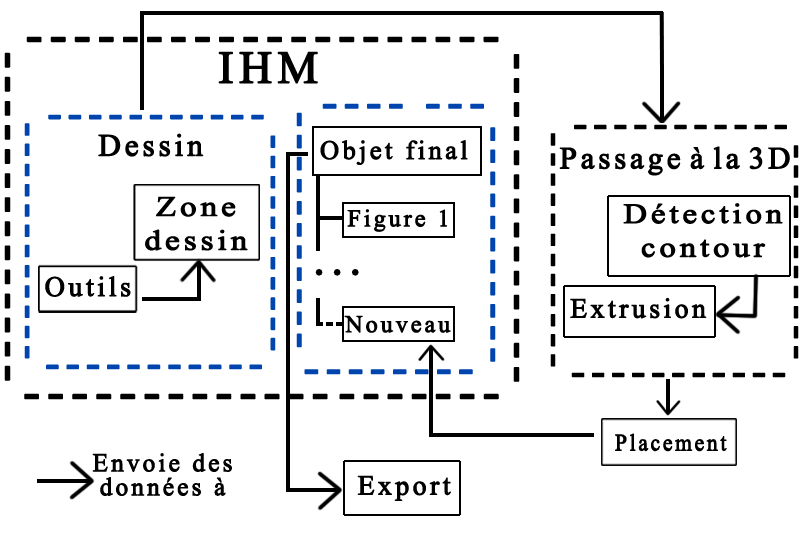
\includegraphics[scale=0.3]{images/archilogi/archi6.png}}
	\end{frame}	
			
	\section{Implémentation sous Unity}
		%Expliquer nos choix par rapports aux objectifs énoncés
			\begin{frame}{Implémentation sous Unity}
				Nous avons défini:
					\begin{itemize}
						\item Choix technologique : Unity
						\item Le fonctionnement de l'application
						\item L'architecture du logiciel
					\end{itemize}
				Implémentation des modules sous Unity
			\end{frame}
		
	\subsection{IHM et Outils}
	\begin{frame}{IHM et Outils}

				\begin{itemize}
					\item Technologie Unity UI (gestion de menus)
					\item Boutons et caméras vides
					\item Facilité d'implémentation de nouveaux outils
				\end{itemize}
				\centerline{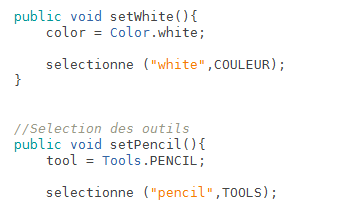
\includegraphics[scale=0.2]{images/Nono/img8.png}}
			
	\end{frame}
	

	\subsection{La zone de dessin}
	\begin{frame}{La zone de dessin}
		Objectif: dessiner sur un plan
			
		Problèmes:
			\begin{itemize}
				\item La zone de dessin et l'écran pas le même référentiel
				
			\end{itemize} 
			Lancé de rayon : 
			Trouver la position du doigt
			\begin{itemize}
				\item Effet de bord
			\end{itemize}
			Vérification de la position du curseur	
		\centerline{
\includegraphics[scale=0.3]{images/Nono/img1.png}}
	\end{frame}
	
	\begin{frame}{La zone de dessin}
			\begin{itemize}
				\item Fond transparent pour la détection de contours
			\end{itemize} 
			Définition d'un fond en alpha (transparence)
			\begin{itemize}
				\item Comment garder un tracé continu ?
			\end{itemize}
			Nous utilisons l'équation cartésienne de la droite :
			\centerline{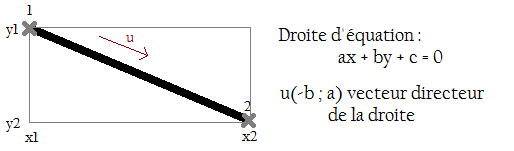
\includegraphics[scale=0.6]{images/intro/trait.png}}
	\end{frame}
	\subsection{Extrusion}
	\begin{frame}{L'extrusion : Définition}
		Plusieurs étapes pour passer d'un dessin à un objet :
		\begin{itemize}
			\item Détection des contours du dessin
			\item Création de meshes
			\item Assemblage des meshes -> Objet 3D
			\item Application de la texture pour rendre l'objet coloré
		\end{itemize}
	
	\end{frame}
		
	\begin{frame}{L'extrusion}
		\centerline{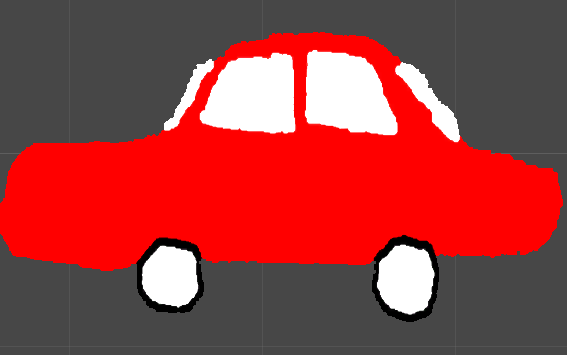
\includegraphics[scale=0.3]{images/techno/voiture.png}
				
\includegraphics[scale=0.3]{images/techno/fleche.png}
				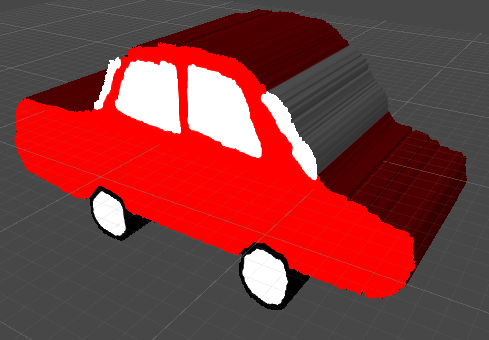
\includegraphics[scale=0.3]{images/techno/voiture3D.png}}
		Passage du dessin à l'objet 3D :
		\begin{itemize}
			\item Détection et extrusion faites par UCLA Mesh Creator
			\item Intégration de l'outil à notre application
		\end{itemize}
		\medbreak
		Problèmes rencontrés :
		\begin{itemize}
			\item Utilisation impossible en mode "Jeu" -> Exécutable impossible
			\item Création de nombreux fichiers inutiles pour la suite
		\end{itemize}
	\end{frame}
	\subsection{Export}
	\begin{frame}{Envoi des données}
		\centerline{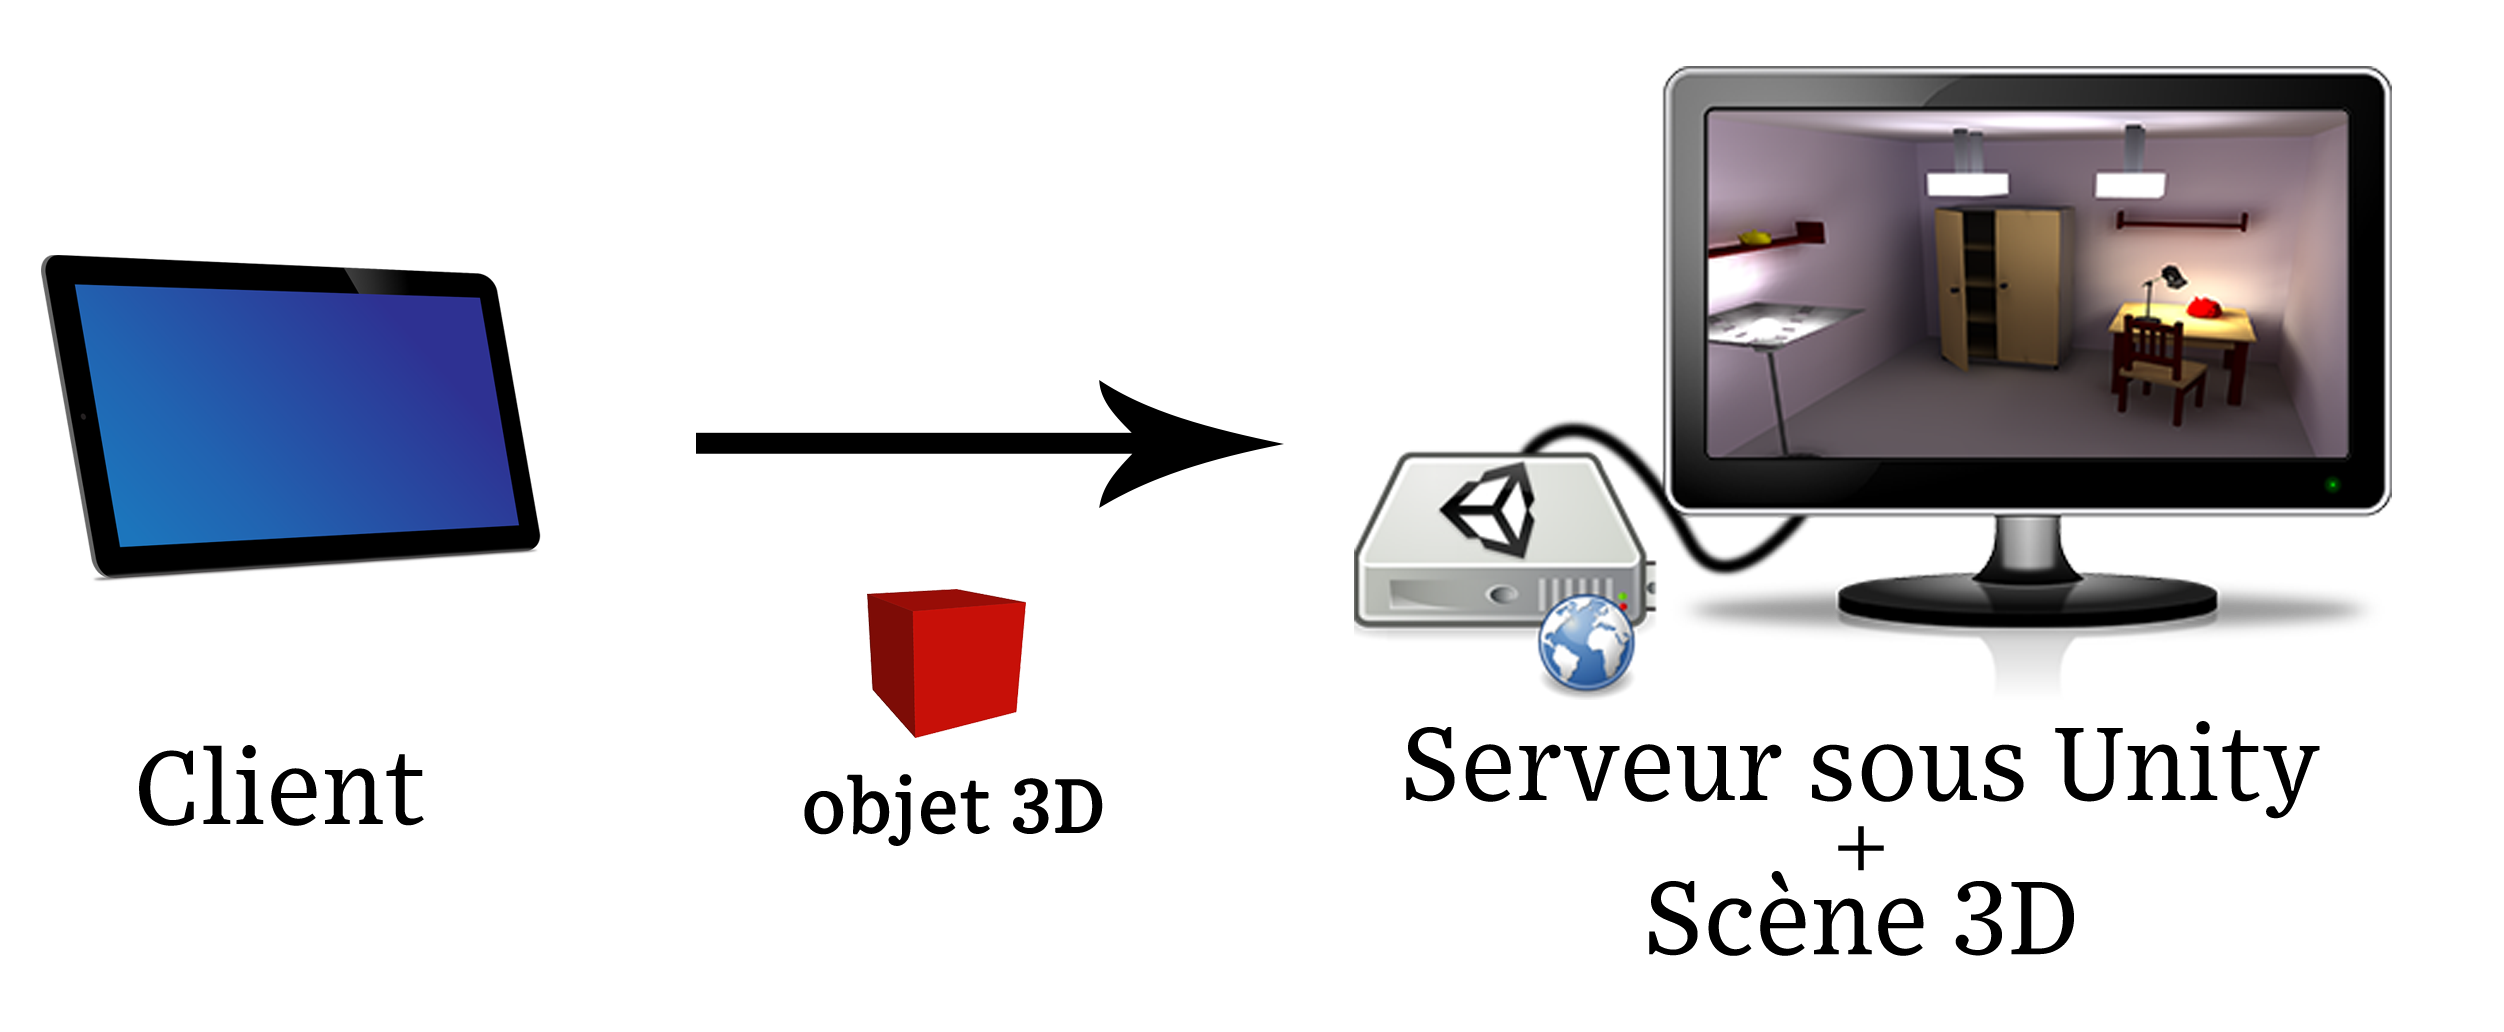
\includegraphics[height=120pt]{images/network/sending_model2.png}}
	\end{frame}
	
	

	\begin{frame}{Côté serveur}
		\centerline{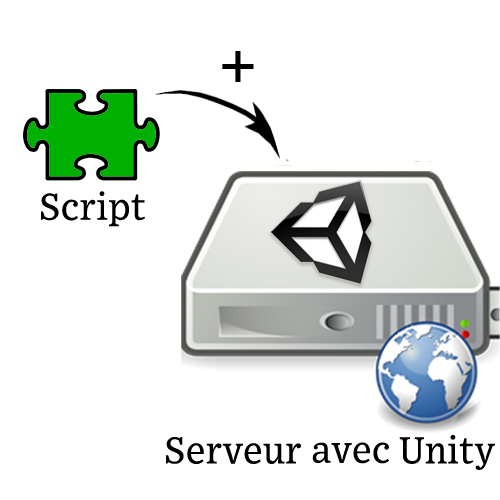
\includegraphics[height=150pt]{images/network/plugin.png}}
		\begin{itemize}	
			\item \pause Simple et modulaire \pause
			\item Reçoit les données \pause
			\item Affiche l'objet 
		\end{itemize}	
		
	\end{frame}
	
	
	\begin{frame}{Socket TCP}
		\centerline{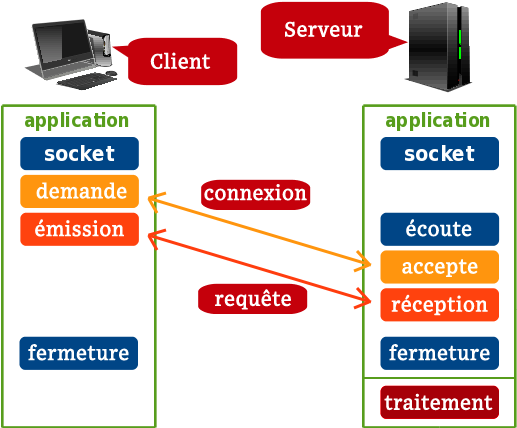
\includegraphics[height=150pt]{images/network/tcp-socket6.png}}
			\begin{itemize}
				\item \pause Protocole de communication universel \pause
				\item Documenté \pause
				\item Permet d'envoyer des octets, donc flexible
			\end{itemize}
	\end{frame}
	
	\section{Conclusion}
	
	\begin{frame}{Notre application}
		Voici une vidéo montrant un exemple d'utilisation de notre application :
		
		\href{run:PresentationAppli.wmv}{
\includegraphics[width=200pt]{images/techno/unity-logo.png}}
	\end{frame}
	
	\begin{frame}{Conclusion}
		Nous avons fait une application Unity :
		\begin{itemize}
			\item \pause Sur tablette Windows\pause
			\item Simple et rapide\pause
		\end{itemize}
		\centerline{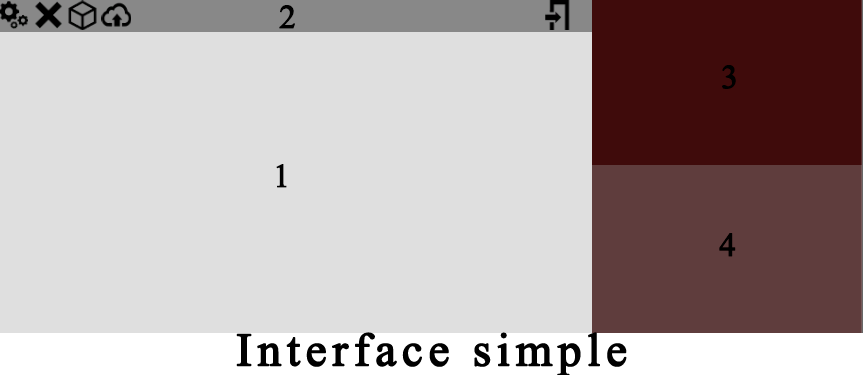
\includegraphics[height=60pt]{images/conclu/menu.png}\pause\hspace{10 mm}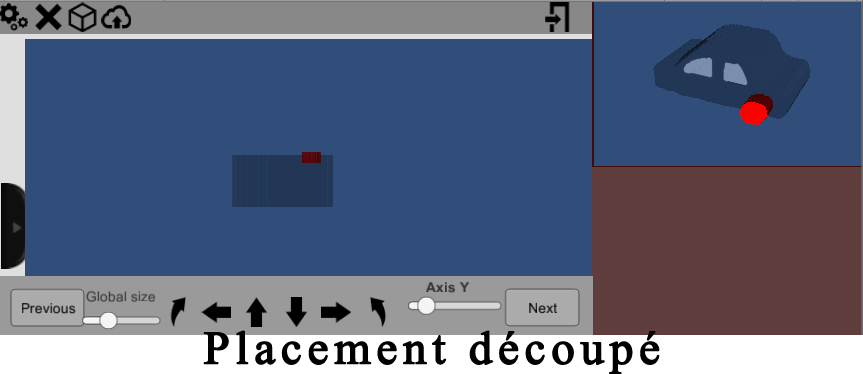
\includegraphics[height=60pt]{images/conclu/place.png}\pause}
		\begin{tabular}{lll}
			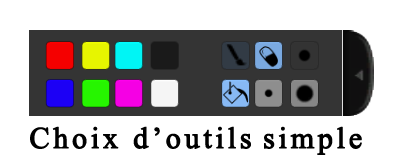
\includegraphics[height=40pt]{images/conclu/outils.png} & \pause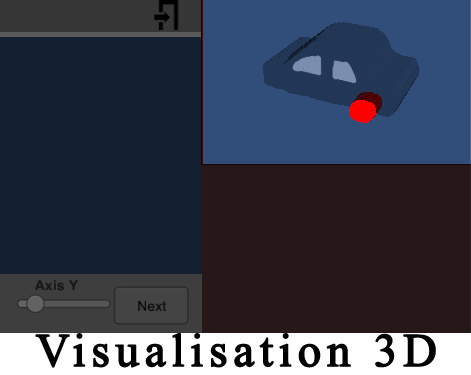
\includegraphics[height=75pt]{images/conclu/visu.png}\pause & 
\includegraphics[height=30pt]{images/conclu/export.png}
		\end{tabular}
		 
	\end{frame}
	
	\begin{frame}{Conclusion}
		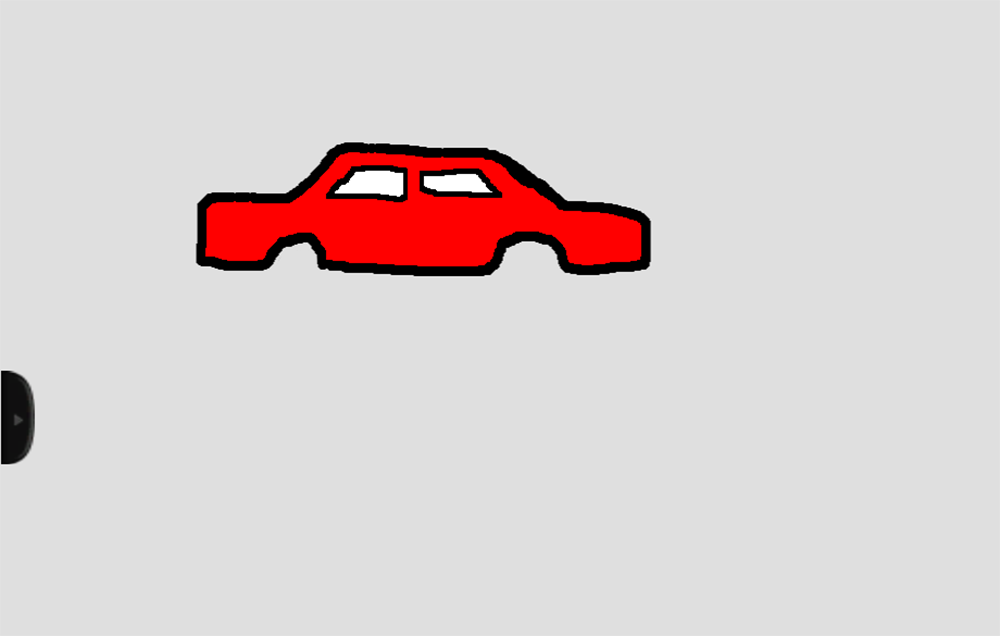
\includegraphics[height=150pt]{images/conclu/avant.png}
	\end{frame}
	\begin{frame}{Conclusion}
		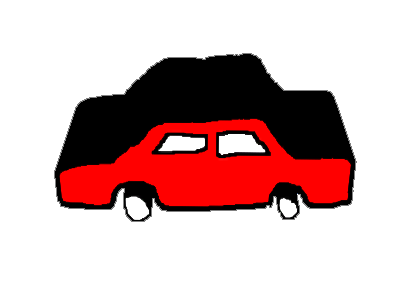
\includegraphics[height=150pt]{images/conclu/apres.png}
	\end{frame}
\end{document}
